\documentclass{article}

\usepackage{amsfonts}
\usepackage{amsmath}
% \usepackage{svg} %For including svgs
% \svgpath{{../assets/}}
\usepackage{graphicx}
\graphicspath{ {../assets/} }
\usepackage[margin=1in]{geometry} %Change margins
\usepackage{hyperref} %For hyperlinks in table of contents and other
\usepackage{float} %For using H in figure
\usepackage{subcaption} %For subfigures
\usepackage{booktabs} %For tables
\usepackage{multirow} %For tables

%\usepackage[charsperline=120]{jlcode} %For Julia Code Listing https://github.com/wg030/jlcode

\addtolength{\jot}{1em} %https://tex.stackexchange.com/questions/14679/amsmath-align-environment-row-spacing

\title{Optimization Assignment 3\\Linear Programs and Applications}
\date{Winter 2021}
\author{Kim Paolo Laberinto (7771083)}

\begin{document}
    \maketitle
    \newpage

    \tableofcontents
    \newpage


    \section{Q1. Linear Programming Applied to Diet Optimizaton}

    \subsection{Problem Set-up}

    In the assignment, a word problem was given in which a diet had to be constructed such that it minimized the total calorie content, while also still meeting the minimum daily nutriential requirements given.

    In this section the word problem will be formulated into linear program consisting of the following elements.
    \begin{itemize}
        \item Variables
        \item Objective Function
        \item Constraints
    \end{itemize}

    \subsubsection{Variables}

    The variables are the number of servings of each food item as denoted in Tab. \ref{tab:Q1_variables}.

    \begin{table}[H]
        \centering
        \begin{tabular}{@{}ll@{}}
        \toprule
        Variable & Description                             \\ \midrule
        $x_1$         & Number of servings of provolone         \\
        $x_2$         & Number of servings of mozzarella        \\
        $x_3$         & Number of servings of 2\% milk          \\
        $x_4$         & Number of servings of salami            \\
        $x_5$         & Number of servings of ham               \\
        $x_6$         & Number of servings of brussel sprouts   \\
        $x_7$         & Number of servings of lettuce           \\
        $x_8$         & Number of servings of french fries      \\
        $x_9$         & Number of servings of orange            \\
        $x_{10}$      & Number of servings of whole wheat bread \\
        $x_{11}$      & Number of servings of bran muffin       \\ \bottomrule
        \end{tabular}
        \caption{Variables for Linear Program for Diet Optimization}
        \label{tab:Q1_variables}
    \end{table}

    \subsubsection{Objective Function}

    Let $E(x_i)$ denote the caloric (energy) content of 1 serving of food $x_i$ in units of kcal (equivalent to in units of food calories (i.e 1 kcal = 1 food calorie)).

    The objective of this linear program is the following. Shown without any constraints.

    \begin{equation}
    \begin{aligned}
        & \underset{\mathbf{x}}{\text{minimize}} & & \sum_{i} E(x_i) x_i \\
    \end{aligned}
    \end{equation}

    \subsubsection{Constraints}

    In this linear program, the constraints are to meet all the daily nutriential values. There are also constraints to ensure that serving portions are non-negative.

    Let the following functions denote the nutritional content of 1 serving of the food $x_i$

    \begin{itemize}
        \item $\text{Protein}(x_i)$ - protein in grams 
        \item $\text{Carb}(x_i)$ - carbohydrates in grams 
        \item $\text{Fat}(x_i)$ - fat in grams
        \item $\text{VitA}(x_i)$ - Vitamin A in REs 
        \item $\text{VitB1}(x_i)$ - Vitamin B1 Thiamin in milligrams 
        \item $\text{VitB2}(x_i)$ - Vitamin B2 Riboflavin in milligrams 
        \item $\text{VitC}(x_i)$ - Vitamin C in milligrams 
        \item $\text{Fibre}(x_i)$ - Fibre in grams 
    \end{itemize}

    Then the linear program can be summarized as the following.

    \begin{equation}
        \begin{aligned}
            & \underset{\mathbf{x}}{\text{minimize}} & & \sum_{i} E(x_i) x_i \\
            & \text{subject to} & & x_i \ge 0, \; i = 1, \ldots, 11 \\
            & & & \sum_{i} \text{Protein}(x_i) x_i \ge 60 \\
            & & & \sum_{i} \text{Carb}(x_i) x_i \ge 300 \\
            & & & \sum_{i} \text{Fat}(x_i) x_i \ge 40 \\
            & & & \sum_{i} \text{VitA}(x_i) x_i \ge 800 \\
            & & & \sum_{i} \text{VitB1}(x_i) x_i \ge 1.0 \\
            & & & \sum_{i} \text{VitB2}(x_i) x_i \ge 1.2 \\
            & & & \sum_{i} \text{VitC}(x_i) x_i \ge 60 \\
            & & & \sum_{i} \text{Fibre}(x_i) x_i \ge 10 \\
        \end{aligned}
    \end{equation}
    

    \subsection{Solution using Julia}

    The linear program was solved using JuMP.jl from the Julia ecosystem, yielding the following solution.

    % Solution
    % Please add the following required packages to your document preamble:
    % \usepackage{booktabs}
    \begin{table}[H]
        \centering
        \begin{tabular}{@{}llrr@{}}
        \toprule
        Variable & Food & Diet Serving Count & Diet Quantity \\ \midrule
        $x_1$    & Provolone         & 0.0  & - \\
        $x_2$    & Mozzarella        & 0.0  & - \\
        $x_3$    & 2\% Milk          & 0.0  & - \\
        $x_4$    & Salami            & 0.0  & - \\
        $x_5$    & Ham               & 0.0  & - \\
        $x_6$    & Brussel Sprouts   & 6.96 & 1740.0 mL \\
        $x_7$    & Lettuce           & 0.0  & - \\
        $x_8$    & French Fries      & 0.0  & - \\
        $x_9$    & Orange            & 2.17 & 2.17 medium \\
        $x_{10}$ & Whole Wheat Bread & 0.0  & - \\
        $x_{11}$ & Bran Muffin       & 10.0 & 10.0 medium \\ \bottomrule
        \end{tabular}
        \caption{Optimized diet solution using Julia. Serving counts, and quantity shown.}
        \label{tab:Q1_Julia_Solution}
    \end{table}

    \begin{table}[H]
        \centering
        \resizebox{\textwidth}{!}{%
        \begin{tabular}{@{}lrrrrrrrrrr@{}}
        \toprule
        &
        Servings &
        \begin{tabular}[c]{@{}r@{}}Energy\\ {[}kcal{]}\end{tabular} &
        \begin{tabular}[c]{@{}r@{}}Protein\\ {[}g{]}\end{tabular} &
        \begin{tabular}[c]{@{}r@{}}Carbs\\ {[}g{]}\end{tabular} &
        \begin{tabular}[c]{@{}r@{}}Fat\\ {[}g{]}\end{tabular} &
        \begin{tabular}[c]{@{}r@{}}Vitamin A\\ {[}RE{]}\end{tabular} &
        \begin{tabular}[c]{@{}r@{}}Vitamin B1\\ {[}mg{]}\end{tabular} &
        \begin{tabular}[c]{@{}r@{}}Vitamin B2\\ {[}mg{]}\end{tabular} &
        \begin{tabular}[c]{@{}r@{}}Vitamin C\\ {[}mg{]}\end{tabular} &
        \begin{tabular}[c]{@{}r@{}}Fibre\\ {[}g{]}\end{tabular} \\ \midrule
        $x_6$ - Brussel Sprouts & 6.96 & 445.44 & 27.84 & 97.44 & 0.0 & 828.24 & 1.25 & 0.90 & 709.92 & 34.8 \\
        $x_8$ - French Fries    & 0.0  & 0.0    & 0.0   & 0.0   & 0.0 & 0.0    & 0.0  & 0.0  & 0.0    & 0.0  \\
        $x_9$ - Oranges         & 2.17 & 134.54 & 2.17  & 32.55 & 0.0 & 60.76  & 0.24 & 0.11 & 151.9  & 5.64 \\
        $x_{11}$ - Bran Muffin  & 10.0 & 1040.0 & 30    & 170   & 40  & 180    & 0.5  & 0.8  & 0.0    & 18   \\ \midrule
        Diet Summary            &      & 1620.0 & 60    & 300   & 40  & 1069   & 2.0  & 1.8  & 861.8  & 58.4 \\ \midrule
        Daily Requirement       &      &        & 60    & 300   & 40  & 800    & 1.0  & 1.2  & 60     & 10   \\ \bottomrule
        \end{tabular}%
        }
        \caption{Nutrition Summary of Optimized Diet using Julia showing all nutritional daily requirements are met. Rounded values for clarity.}
        \label{tab:Q1_NutritionSummary_Solution_Julia}
    \end{table}

    \subsection{Solution using Matlab}

    The linear program was solved using Matlab, yielding the following solution.

    % Solution

    \subsection{Observations}

    There are several observations to make from these solutions.

    %Observations
    \begin{itemize}
        \item 
    \end{itemize}

    \subsection{Follow-up Question and Solution - Doubling Calories in Bran Muffins}

    A follow up question in the assignment was to determine what happens to the diet if the calories in the muffins are increased by a factor of 2.

    Using this new calorie content for the bran muffins yields the following solution.

    % Solution

    \begin{table}[H]
        \centering
        \begin{tabular}{@{}llrr@{}}
        \toprule
        Variable & Food & Diet Serving Count & Diet Quantity \\ \midrule
        $x_1$    & Provolone         & 0.0  & - \\
        $x_2$    & Mozzarella        & 0.0  & - \\
        $x_3$    & 2\% Milk          & 0.0  & - \\
        $x_4$    & Salami            & 0.0  & - \\
        $x_5$    & Ham               & 0.0  & - \\
        $x_6$    & Brussel Sprouts   & 11.96 & 2990 mL \\
        $x_7$    & Lettuce           & 0.0  & - \\
        $x_8$    & French Fries      & 5.0  & 50 strips \\
        $x_9$    & Orange            & 2.17 & 2.17 medium \\
        $x_{10}$ & Whole Wheat Bread & 0.0  & - \\
        $x_{11}$ & Bran Muffin       & 0.0 & - \\ \bottomrule
        \end{tabular}
        \caption{Optimized diet solution, where bran muffins had 2x calories. Serving counts, and quantity shown. (Solution found using Julia). }
        \label{tab:Q1_doublecalmuffins_solution}
    \end{table}

    \begin{table}[H]
    \centering
    \resizebox{\textwidth}{!}{%
    \begin{tabular}{@{}lrrrrrrrrrr@{}}
    \toprule
     &
      Servings &
      \begin{tabular}[c]{@{}r@{}}Energy\\ {[}kcal{]}\end{tabular} &
      \begin{tabular}[c]{@{}r@{}}Protein\\ {[}g{]}\end{tabular} &
      \begin{tabular}[c]{@{}r@{}}Carbs\\ {[}g{]}\end{tabular} &
      \begin{tabular}[c]{@{}r@{}}Fat\\ {[}g{]}\end{tabular} &
      \begin{tabular}[c]{@{}r@{}}Vitamin A\\ {[}RE{]}\end{tabular} &
      \begin{tabular}[c]{@{}r@{}}Vitamin B1\\ {[}mg{]}\end{tabular} &
      \begin{tabular}[c]{@{}r@{}}Vitamin B2\\ {[}mg{]}\end{tabular} &
      \begin{tabular}[c]{@{}r@{}}Vitamin C\\ {[}mg{]}\end{tabular} &
      \begin{tabular}[c]{@{}r@{}}Fibre\\ {[}g{]}\end{tabular} \\ \midrule
    $x_6$ - Brussel Sprouts & 11.96 & 765.44 & 47.84 & 167.44 & 0.0  & 1423.24 & 2.1582 & 1.55 & 1219.92 & 59.80 \\
    $x_8$ - French Fries    & 5     & 790    & 10.0  & 100.0  & 40.0 & 0       & 0.45   & 0.05 & 25.0    & 0     \\
    $x_9$ - Oranges         & 2.17  & 134.54 & 2.17  & 32.55  & 0.0  & 60.76   & 0.24   & 0.11 & 151.9   & 5.64  \\
    $x_{11}$ - Bran Muffin  & 0.0   & 0.0    & 0.0   & 0.0    & 0.0  & 0.0     & 0.0    & 0.0  & 0.0     & 0.0   \\ \midrule
    Diet Summary            &       & 1690   & 60    & 300    & 40   & 1484    & 2.8    & 1.7  & 1396.8  & 65.4  \\ \midrule
    Daily Requirement       &       &        & 60    & 300    & 40   & 800     & 1.0    & 1.2  & 60      & 10    \\ \bottomrule
    \end{tabular}%
    }
    \caption{Nutritional Summary of Diet (double calorie muffins).}
    \label{tab:Q1_doublecalmuffins_nutritionsummary}
    \end{table}

    There are several observations to make from this new solution:

    %Observations
    \begin{itemize}
        \item 
    \end{itemize}


    \section{Q2. Example of Conversion to Standard Form}

    \section{Q3. Example of Graphically Solving a Linear Program}

    \begin{figure}[H]
        \centering
        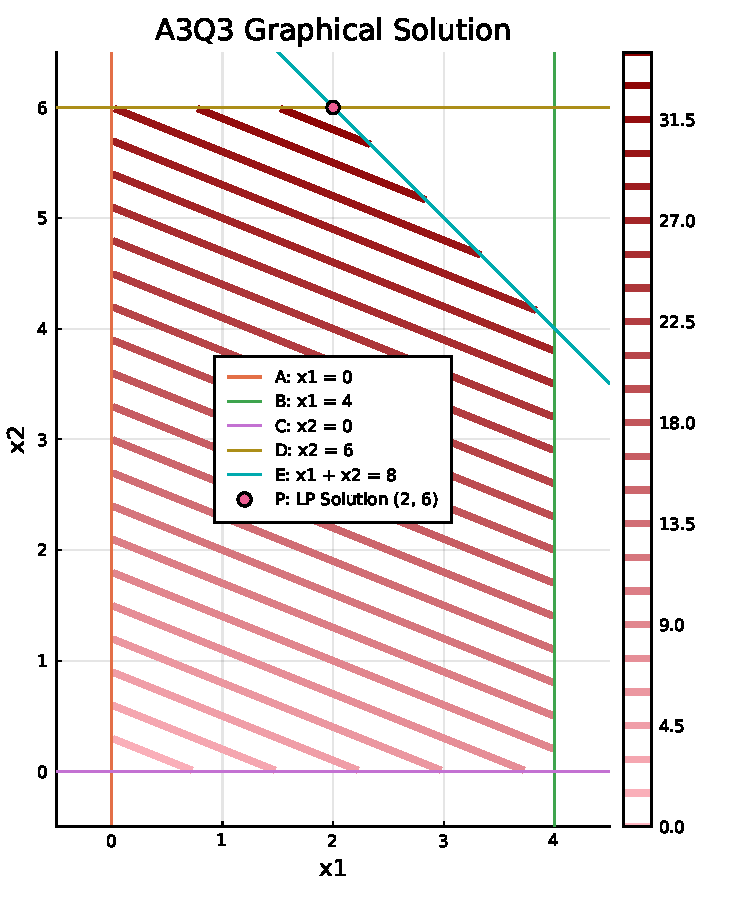
\includegraphics[width=0.5\linewidth]{A3Q3_Plot.pdf}
        \caption{Graphical Solution to A3Q3 question, showing feasible region, objective contours, and solution.}
        \label{fig:A3Q3_GraphicalSolution}
    \end{figure}

    \section{Q4. Textbook Questions}

    \subsection{12.9}

    \subsection{12.15}

    \subsection{12.21}

    \subsection{12.22}


    \newpage
    \appendix

    \section{Source Code}

\end{document}